\documentclass[tikz,border=10pt]{standalone}
\usetikzlibrary{calc}

\begin{document}
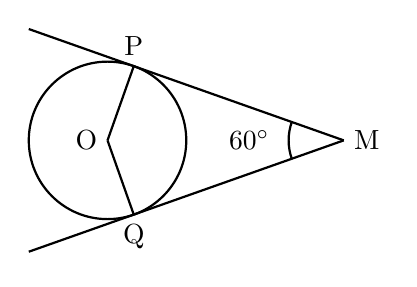
\begin{tikzpicture}[scale=1, thick]
    % 1. Define Coordinates
    \coordinate (O) at (0,0);
    \coordinate (M) at (3,0);

    % Tangent points for a 1cm radius circle with M at (3,0)
    % Angle alpha = arcsin(1/3) approx 19.47 degrees
    \coordinate (P) at ({1/3}, {sqrt(8)/3});
    \coordinate (Q) at ({1/3}, {-sqrt(8)/3});

    % 2. Draw the Circle
    \draw (O) circle (1cm);

    % 3. Draw Tangent Lines MP and MQ (extending past P and Q)
    \draw (M) -- ($(M)!1.5!(P)$);
    \draw (M) -- ($(M)!1.5!(Q)$);

    % 4. Draw the Radii OP and OQ
    \draw (O) -- (P);
    \draw (O) -- (Q);

    % 5. Add Point Labels
    \node[left] at (O) {O};
    \node[right] at (M) {M};
    \node[above] at (P) {P};
    \node[below] at (Q) {Q};

    % 6. DRAW THE ARC MANUALLY (Guarantees no circle)
    % This starts exactly on the line MQ and ends exactly on MP
    \draw ($(M) + (199.47:0.7cm)$) arc (199.47:160.53:0.7cm);

    % 7. Place the 60 degree text beside the arc
    \node at ($(M)+(-1.2,0)$) {$60^\circ$};

\end{tikzpicture}
\end{document}
